\usepackage{pgf}
\usepackage{tikz}
\usetikzlibrary{arrows,automata}

\newcommand{\ejemplografo}{
\begin{tikzpicture}[--,>=stealth',shorten >=1pt,auto,node distance=3cm,semithick]
  \tikzstyle{every state}=[draw=black,text=black]

  \node[state]         (A)                    {$A$};
  \node[state]         (B)      [right of=A]  {$B$};
  \node[state]         (C)      [below of=A]  {$C$};
  \node[state]         (D)      [right of=C]  {$D$};
  
  \path (B) edge  [bend left]  node   (D);
%            edge               node   (B)
 %           edge               node   (C)
%        (B) edge               node   (C);

\end{tikzpicture}}


\newcommand{\ejemplomarkov}{
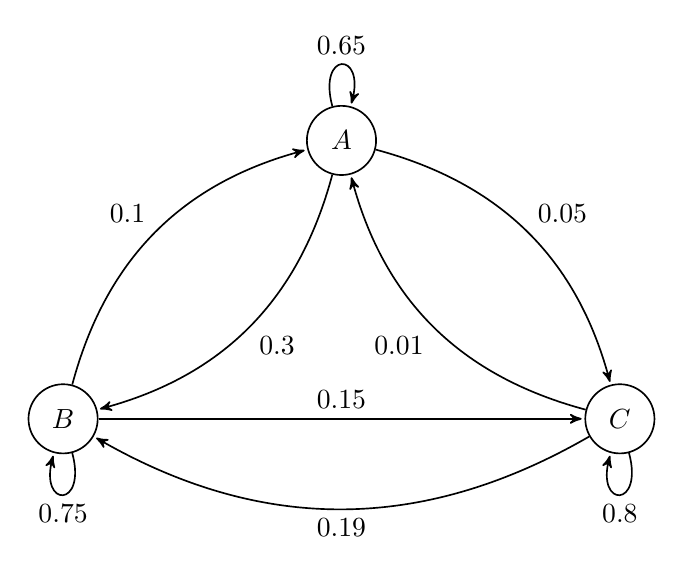
\begin{tikzpicture}[->,>=stealth',shorten >=1pt,auto,node distance=5cm,semithick]
  \tikzstyle{every state}=[draw=black,text=black]

  \node[state]         (A)                    {$A$};
  \node[state]         (B) [below left of=A]  {$B$};
  \node[state]         (C) [below right of=A] {$C$};
  
  \path (A) edge  [loop above] node {$0.65$} (A)
            edge  [bend left]  node {$0.3$}  (B)
            edge  [bend left]  node {$0.05$} (C)
        (B) edge  [loop below] node {$0.75$} (B)
            edge  [bend left]  node {$0.1$}  (A)
            edge               node {$0.15$} (C)
        (C) edge  [loop below] node {$0.8$}  (C)
            edge  [bend left]  node {$0.01$} (A)
            edge  [bend left]  node {$0.19$} (B);
\end{tikzpicture}}

\newcommand{\ejemplomarkovcompleto}{
\begin{tikzpicture}[->,>=stealth',shorten >=1pt,auto,node distance=5cm,semithick]
  \tikzstyle{every state}=[draw=black,text=black]

  \node[state]         (S)                    {$S$};
  \node[state]         (H)      [right of=A]  {$H$};
  
  \path (S) edge  [loop above] node {$0.5$}  (S)
            edge  [bend left]  node {$0.5$}  (H)
        (H) edge  [loop below] node {$0.75$} (H)
            edge  [bend left]  node {$0.25$} (S);

\end{tikzpicture}}

